\documentclass{article}[12pt]
\usepackage[utf8]{inputenc}
\usepackage{amsmath}
\usepackage{amsfonts}
\usepackage{siunitx}
\usepackage{graphicx}
\usepackage{hyperref}

\sisetup{per-mode=symbol}
\hypersetup{
    colorlinks=true,
    linkcolor=blue,
    filecolor=magenta,
    urlcolor=blue
}

\title{Microelectronic Circuits Assignment 1}
\author{Sai Kartik (2020A3PS0435P)\\ Manpreet Singh (2020A3PS0419P)\\ Rajeev Rajagopal (2020A3PS1237P)}
\date{February, 2022}

\begin{document}
\maketitle
\section*{Question 1}
Value of components (resistor/capacitor) present in the circuit:
\begin{table}[ht]
    \centering
    \caption{Calculated values for question 1}
    \begin{tabular}{|c | c | c|}
        \hline
        Sl. No. & Component Name & Value       \\
        \hline
        1       & R1(k$\Omega$)  & 15k$\Omega$ \\ %last digit of first group member ID+10=5+10=15
        2       & C1 (nF)        & 1nF         \\ %0.1*(last digit of 3rd group member ID+tut sec number) = 0.1*(7+3)=1
        \hline
    \end{tabular}
    \label{tab:values1}
\end{table}
\subsection*{Circuit as on LT SPICE}
%add circuit diagram
\begin{figure}[ht]
    \centering
    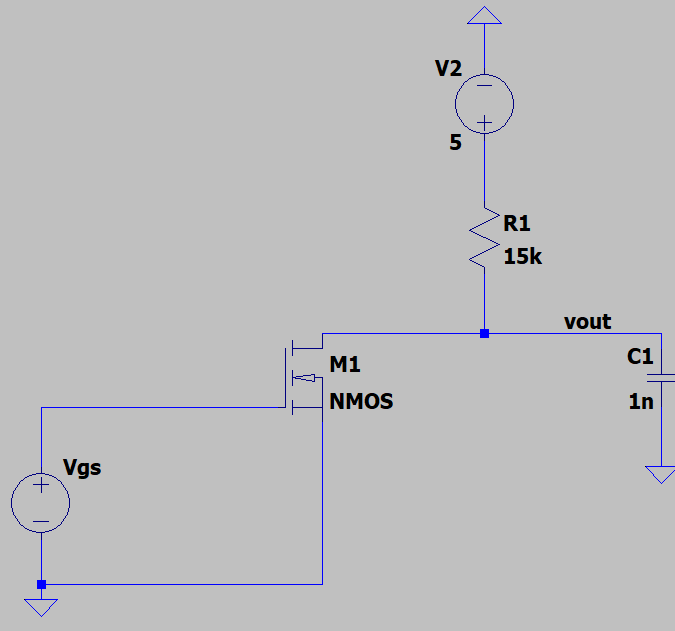
\includegraphics[scale=0.50]{resources/q1.png}
    \caption{Circuit for question 1}
    \label{fig:circuit1}
\end{figure}
\subsection*{Graphs}
%add graphs: frequency response, input, output and transfer characteristics
\newpage
\subsection*{Miscellaneous calculations}
%find DC operating point, small signal equivalent
\subsubsection*{DC operating point}
Given the overdrive voltage of the MOSFET as 0.2V and the threshold voltage as 0.6696061V, to calculate the DC operating point, we must take\\
$V_{GS}=V_{TH}+V_{OV}=0.8696061$V. With this value of $V_{GS}$, the simulation yields the following values:
\begin{figure}[ht]
    \centering
    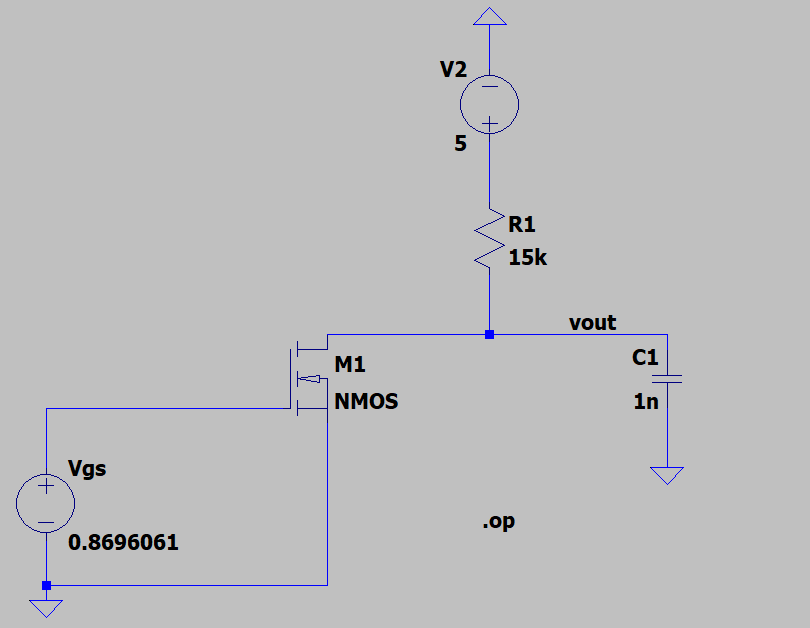
\includegraphics[scale=0.50]{resources/dcop.png}
    \caption{DC operating point circuit}
    \label{fig:dc_op}
\end{figure}
\begin{figure}[ht]
    \centering
    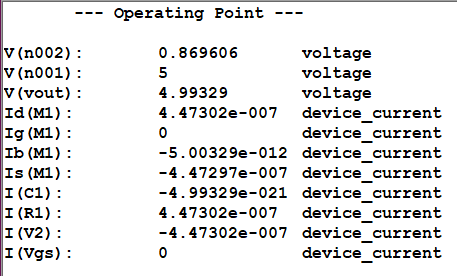
\includegraphics[scale=0.70]{resources/opparams.png}
    \caption{DC operating point parameters}
    \label{fig:dc_op_freq}
\end{figure}
\newpage
\subsubsection*{Small signal calculations}
Transconductance $g_m$ is given by:
$$g_m=\frac{2I_D}{V_{OV}}$$
Using the values found above from the DC operating point calculations, we can calculate the transconductance to be
$$g_m=\frac{2\times4.47302\times10^{-7}}{0.2}=4.47302\times10^{-6}A/V$$
The value of the output resistance $r_0$ corresponding to the early effect/channel length modulation is given by:
$$r_0=\left(\left.\frac{\partial i_D}{\partial V_{DS}}\right)^{-1}\right|_{V_{GS}=\mathrm{constant}}$$
This can be found out from the simulation by setting $V_{GS}=V_{TH}+V_{OV}$ and finding the value of the differential at $V_{DS}=5$V.
\begin{figure}[ht]
    \centering
    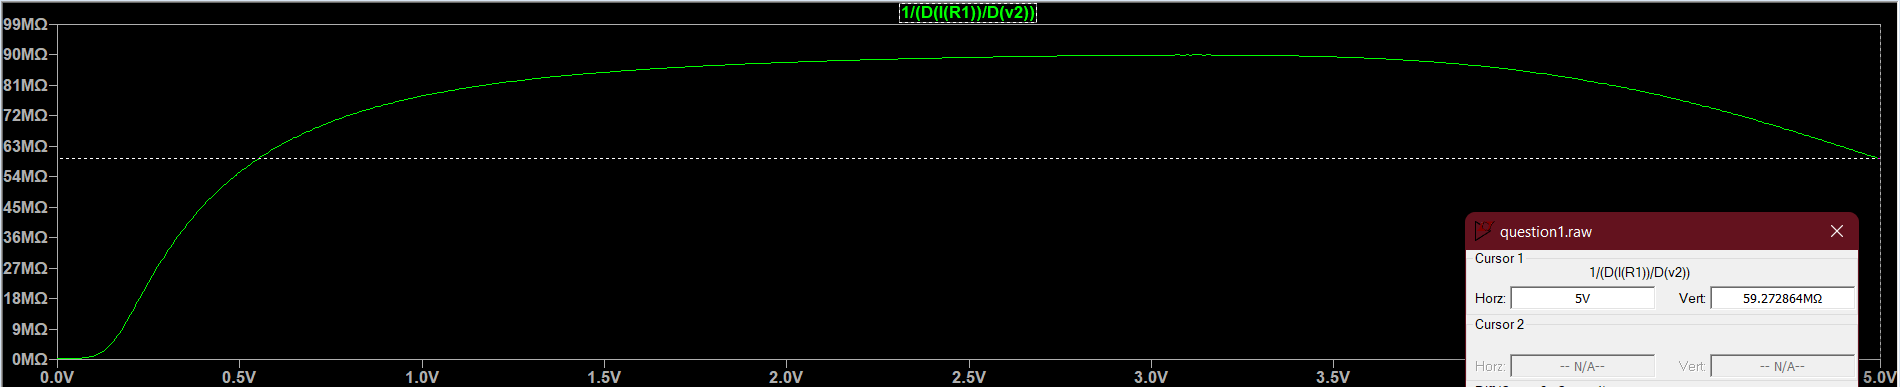
\includegraphics[scale=0.35]{resources/r0.png}
    \caption{Output resistance for small signal calculations}
    \label{fig:r0}
\end{figure}\\
The value of $r_0$ we get from this graph is $r_0=59.272865\mathrm{M}\Omega$.
Collectively, we get the small signal model as:
\begin{figure}[ht]
    \centering
    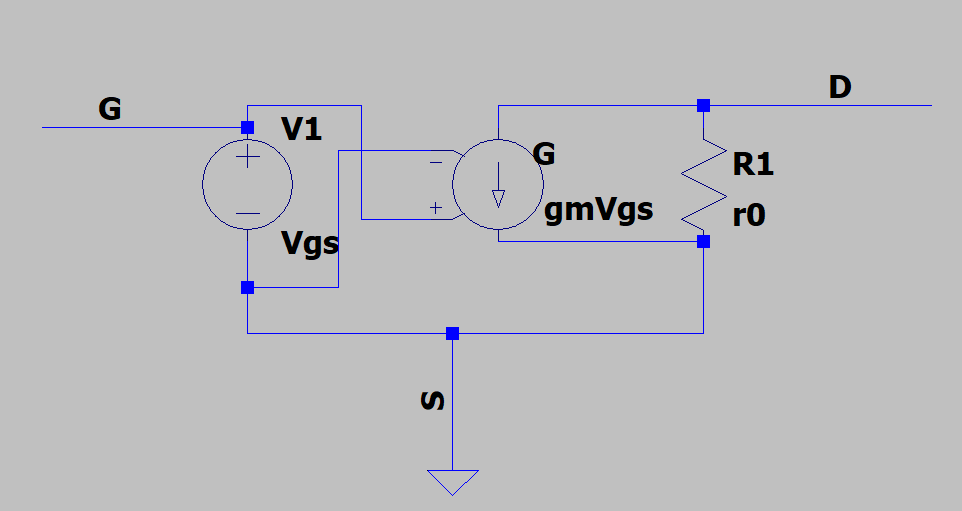
\includegraphics[scale=0.35]{resources/ssmodel.png}
    \caption{Small signal model}
    \label{fig:small_signal}
\end{figure}
\newpage
\section*{Question 2}
Value of components (resistors/gain) present in the circuit
\begin{table}[ht]
    \centering
    \caption{Calculated values for question 2}
    \begin{tabular}{|c | c | c|}
        \hline
        Sl. No. & Component Name   & Value               \\
        \hline
        1       & $R_1$(k$\Omega$) & 30k$\Omega$         \\ %(last digit of 3rd group member ID+3) * tut section = (7+3)*3 = 30
        2       & $R_2$(k$\Omega$) & 17k$\Omega$         \\ %product of last two digits of 1st group member ID + tut section = (3*5)+2=17
        3       & $R_3$(k$\Omega$) & 30k$\Omega$         \\ %sum of last three digits of 2nd group member ID % 8)* tut section = (4+1+9)%8*3=30
        4       & $R_4$(k$\Omega$) & 50k$\Omega$         \\ %product of last two digits of 3rd group member ID + tut section = (7+3)*3 = 30
        5       & k                & 18 \si{\volt/\volt} \\ %last 2 digits of 1st group member admission year - tut section = 20-2=18
        \hline
    \end{tabular}
    \label{tab:values2}
\end{table}
\subsection*{Circuit as on LT SPICE}

\begin{figure}[ht]
    \centering
    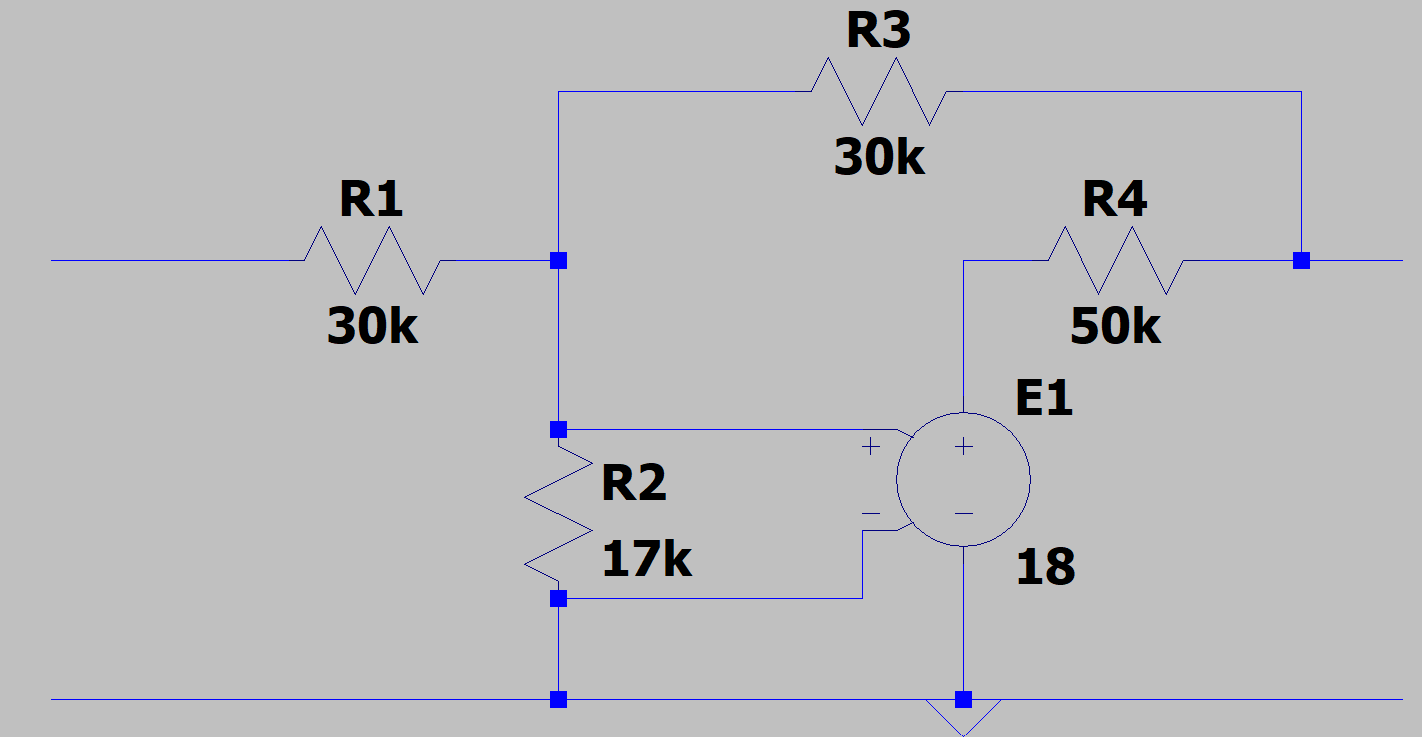
\includegraphics[scale=0.25]{resources/orgcircuit.png}
    \caption{Original 2 port network simulated on LT SPICE}
\end{figure}
\newpage
\subsection*{Z, Y and H Parameters}
%add Z, Y and h parameters
\subsubsection*{Z parameters}
Z parameters as obtained from LT SPICE
$$ Z = \begin{bmatrix}
        23.492822k\Omega & -4.0669856k\Omega \\
        -47.99043k\Omega & -11.24402k \Omega
    \end{bmatrix}
$$
\subsubsection*{Y parameters}
Y parameters as obtained from LT SPICE
$$ Y = \begin{bmatrix} %fill matrix with proper values
        24.479166\mu\mho  & -8.8541665\mu\mho \\
        -104.47916\mu\mho & -51.145835\mu\mho
    \end{bmatrix}
$$
\subsubsection*{H parameters}
$$ H = \begin{bmatrix} %fill matrix with proper values
        40.851062k\Omega       & 361.70211m \mathrm{V/V} \\
        -4.268085 \mathrm{A/A} & -88.936169\mho
    \end{bmatrix}
$$
\newpage
\subsection*{Calculations}
%add hand calculations of Z, Y and h parameters
\subsubsection*{Z parameters}
\begin{figure}[ht]
    \centering
    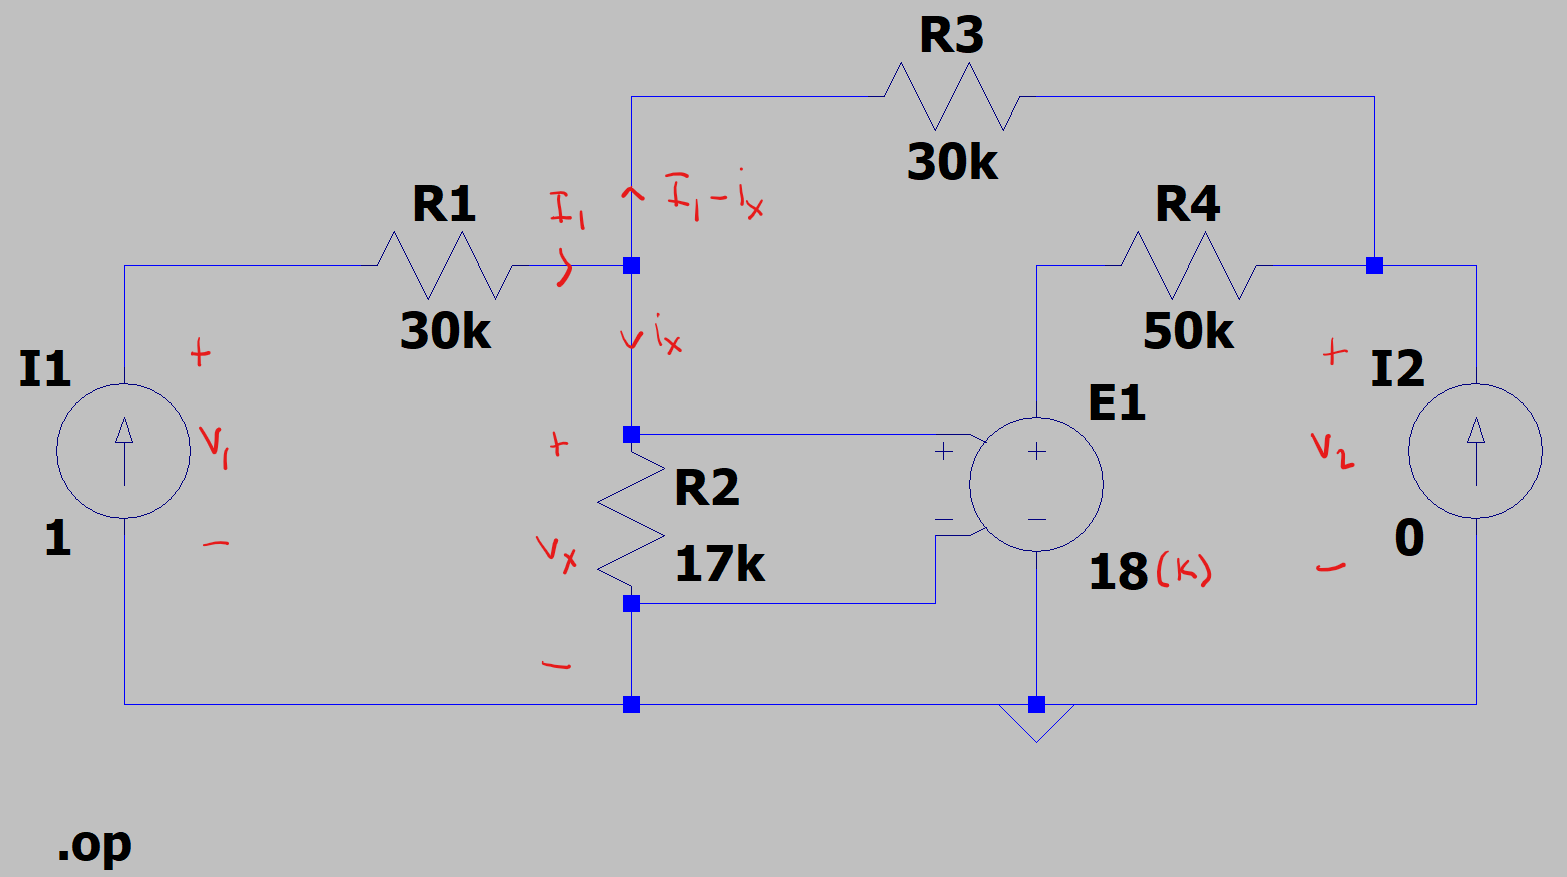
\includegraphics[scale=0.20]{resources/zparams1.png}
    \caption{Z parameter circuit 1 (for $z_{11}$ and $z_{21}$)}
\end{figure}
Assume the convention in the above circuit for the calculations that follow
\begin{gather*}
    -(I_1-i_x)(R_3+R_4)-kV_x+V_x=0\\
    (i_x-I_1)(R_3+R_4)=V_x(k-1)\\
    (i_x-I_1)(R_3+R_4)=i_xR_2(k-1)\\
    i_x(R_3+R_4-R_2(k-1))=I_1(R_3+R_4)\\
    \implies i_x=I_1\frac{(R_3+R_4)}{R_3+R_4-R_2(k-1)} \\
    V_1=I_1R_1+V_x\\
    V_1=I_1R_1+i_xR_2\\
    V_1=I_1\left[R_1+\frac{R_2(R_3+R_4)}{R_3+R_4-R_2(k-1)}\right] \\
    \implies \frac{V_1}{I_1}=\boxed{z_{11} = R_1 + \frac{R_2(R_3+R_4)}{R_3+R_4-R_2(k-1)}} \\
    \mathrm{Also:} \\
    V_2=(I_1-i_x)R_4+kV_x\\
    V_2=(I_1-i_x)R_4+ki_xR_2\\
    V_2=i_x(kR_2-R_4)+I_1R_4\\
    V_2=I_1\left[R_4+\frac{(kR_2-R_4)(R_3+R_4)}{R_3+R_4+R_2(k-1)}\right]\\
    \implies\frac{V_2}{I_1} = \boxed{z_{21} = R_4 + \frac{(kR_2-R_4)(R_3+R_4)}{R_3+R_4-R_2(k-1)}}
\end{gather*}
\newpage
\begin{figure}[ht]
    \centering
    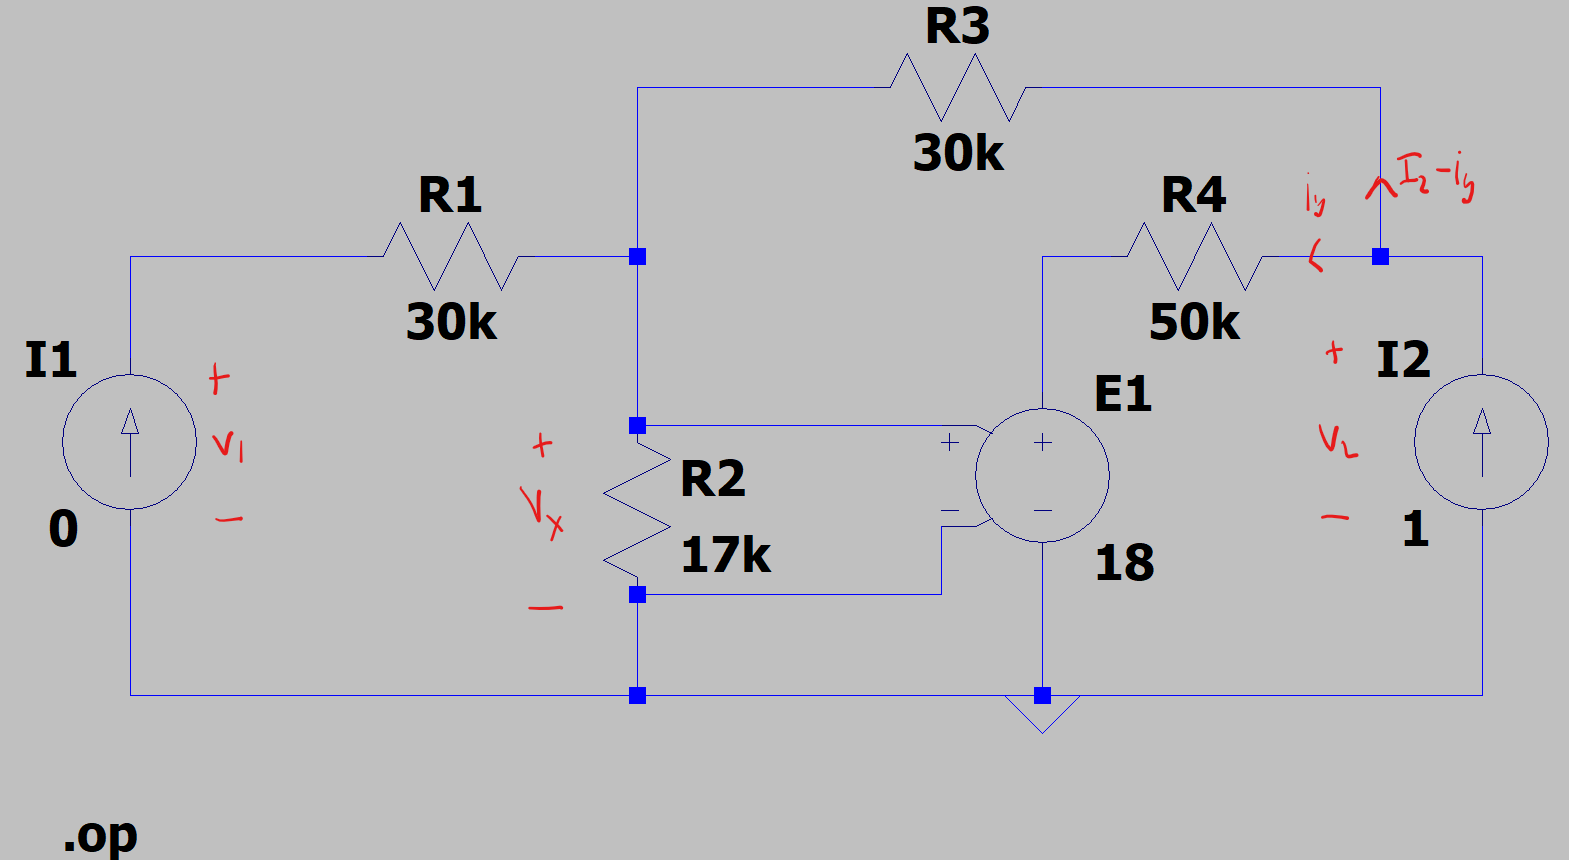
\includegraphics[scale=0.25]{resources/zparams2.png}
    \caption{Z parameter circuit 2 (for $z_{12}$ and $z_{22}$)}
\end{figure}
Assume the convention in the above circuit for the calculations that follow
\begin{gather*}
    -R_3(I_2-i_y)-V_x+kV_x+i_yR_4=0\\
    i_yR_4-R_3(I_2-i_y)=(1-k)V_x\\
    i_yR_4-R_3(I_2-i_y)=(1-k)(I_2-i_y)R_2\\
    i_yR_4=(I_2-i_y)[(1-k)R_2+R_3]\\
    (R_4+R_3+(1-k)R_2)i_y=I_2[(1-k)R_2+R_3]\\
    \implies i_y=I_2\frac{(1-k)R_2+R_3}{(1-k)R_2+R_3+R_4}\\
    V_2=i_yR_4+kV_x\\
    V_2=i_yR_4+k(I_2-i_y)R_2\\
    V_2=i_y[R_4-kR_2]+KI_2R_2\\
    V_2=I_2\left[\frac{(R_4-kR_2)\{(1-k)R_2+R_3\}}{(1-k)R_2+R_3+R_4}+kR_2\right]\\
    \implies \frac{V_2}{I_2} = \boxed{z_{22} = \frac{(R_4-kR_2)\{(1-k)R_2+R_3\}}{(1-k)R_2+R_3+R_4}+kR_2}\\
    \mathrm{Also:} \\
    V_1=V_x=(I_2-i_y)R_2\\
    V_1=I_2R_2\left[1-\frac{(1-k)R_2+R_3}{(1-k)R_2+R_3+R_4}\right]\\
    \implies \frac{V_1}{I_2} = \boxed{z_{12} = R_2\left[1-\frac{(1-k)R_2+R_3}{(1-k)R_2+R_3+R_4}\right]}
\end{gather*}
\newpage
Using the corresponding values taken from \hyperref[tab:values2]{\ref{tab:values2}} into the above equations, we get the matrix for the Z parameters:
$$ Z = \begin{bmatrix}
        23.49282297k\Omega  & -4.066985646k\Omega  \\
        -47.99043062k\Omega & -11.244041914k\Omega
    \end{bmatrix}
$$
Which is in accordance with the values obtained from the simulation.
\subsubsection*{Y parameters}
From the above matrix for Z parameters, we can calculate the Y parameters as follows:
\begin{gather*}
    \Delta Z = z_{11}z_{22}-z_{12}z_{21}\\
    \implies \Delta Z = [(23.49282297\times-11.244041914)-(-47.99043062\times-4.066985646)]\times 10^3\\
    \Delta Z =-459.326\times 10^6\\
    Y = \begin{bmatrix}
        \dfrac{z_{22}}{\Delta Z}  & -\dfrac{z_{12}}{\Delta Z} \\[2ex]
        -\dfrac{z_{21}}{\Delta Z} & \dfrac{z_{11}}{\Delta Z}  \\[2ex]
    \end{bmatrix}
\end{gather*}
Simplifying the above matrix, we get the Y parameters:
$$ Y = \begin{bmatrix}
        2.448 \times 10^{-5}\mu\mho    & -8.8541\times10^{-6}\mu\mho \\[1ex]
        -1.104480\times 10^{-4}\mu\mho & -5.11\times 10^{-5}\mu\mho  \\[1ex]
    \end{bmatrix}
$$
\subsubsection*{H parameters}

Similarly, we can calculate the H parameters as follows:
\begin{gather*}
    H = \begin{bmatrix}
        \dfrac{\Delta Z}{z_{22}} & -\dfrac{z_{12}}{z_{22}} \\[2ex]
        -\dfrac{z_{21}}{z_{22}}  & \dfrac{1}{z_{22}}       \\[2ex]
    \end{bmatrix}
\end{gather*}
Simplifying the above matrix, we get the H parameters:
$$ H = \begin{bmatrix}
        40.8507k\Omega      & -0.3617 \mathrm{V/V} \\[1ex]
        -4.2681\mathrm{A/A} & -88.9363\mho         \\[1ex]
    \end{bmatrix}
$$
\newpage
\subsection*{Load resistance value at port 2}
%calculate according to question given
Varying the output resistance at the terminals of port 2 and by calculating the voltage and current across the resistance, we can calculate the maximum power dissipated across the resistance.
This can be seen in the following figure:
\begin{center}
    \begin{figure}[ht]
        \centering
        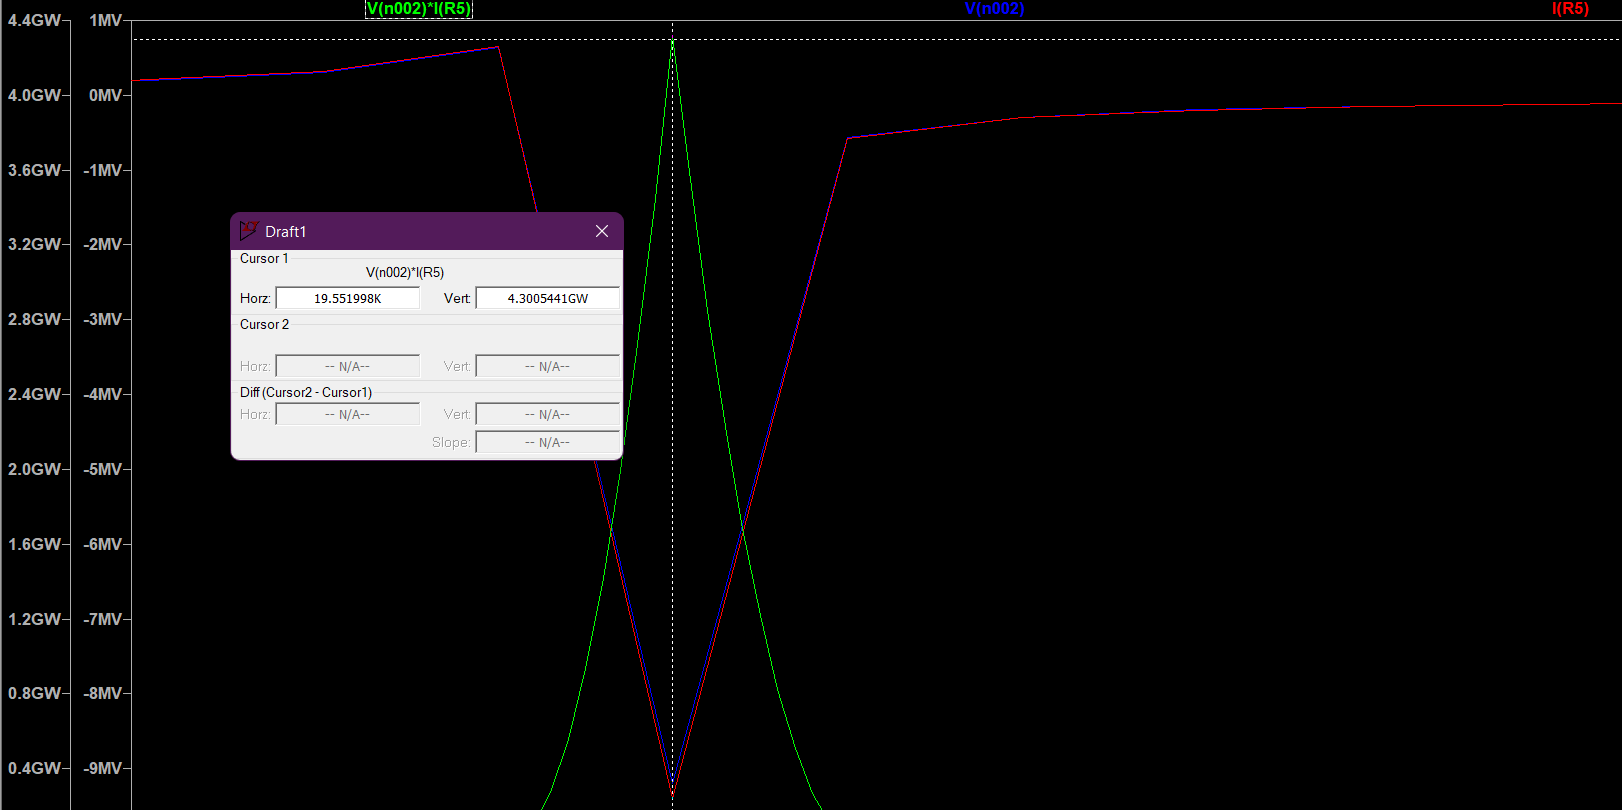
\includegraphics[scale=0.50]{resources/loadresistance.png}
        \caption{Load resistance value at port 2}
    \end{figure}
\end{center}
According to the simulation results shown above, the value for the resistance at which maximum power transfer occurs is $19.551998K\Omega$ and the maximum power transferred is $4.3005441G$W.

\end{document}